\section{Buffer\-Base Class Reference}
\label{classBufferBase}\index{BufferBase@{BufferBase}}
Inheritance diagram for Buffer\-Base::\begin{figure}[H]
\begin{center}
\leavevmode
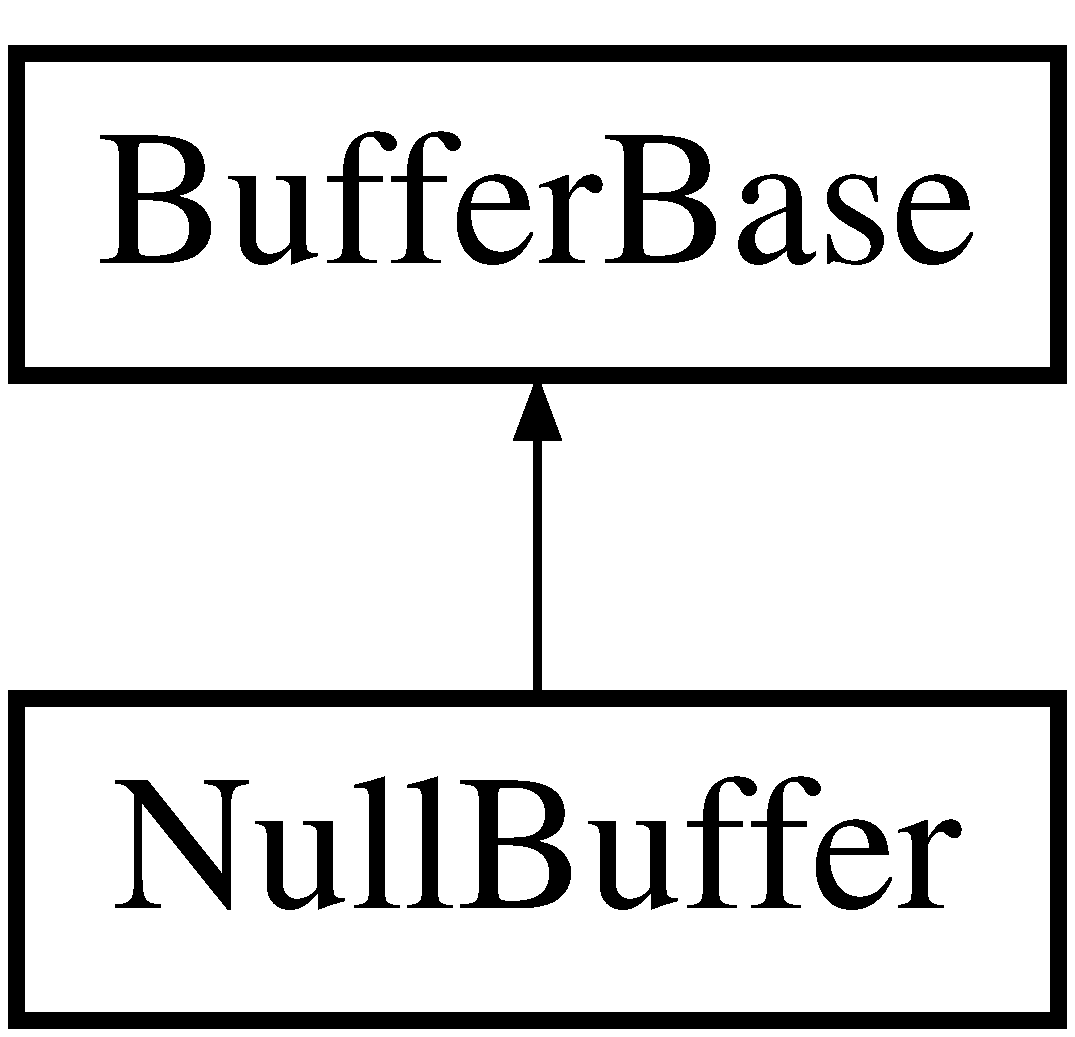
\includegraphics[height=2cm]{classBufferBase}
\end{center}
\end{figure}
\subsection*{Public Member Functions}
\begin{CompactItemize}
\item 
{\bf \_\-\_\-init\_\-\_\-} ()
\item 
{\bf length} ()
\begin{CompactList}\small\item\em Get the buffer length. \item\end{CompactList}\item 
{\bf write} (value)
\begin{CompactList}\small\item\em Write data into the buffer. \item\end{CompactList}\item 
{\bf read} (value)
\begin{CompactList}\small\item\em Read data from the buffer. \item\end{CompactList}\item 
{\bf is\-Full} ()
\begin{CompactList}\small\item\em True if the buffer is full, else false. \item\end{CompactList}\item 
{\bf is\-Empty} ()
\begin{CompactList}\small\item\em True if the buffer is empty, else false. \item\end{CompactList}\item 
{\bf put} (data)
\begin{CompactList}\small\item\em Write data into the buffer. \item\end{CompactList}\item 
{\bf get} ()
\begin{CompactList}\small\item\em Get data from the buffer. \item\end{CompactList}\item 
{\bf get\-Ref} ()
\begin{CompactList}\small\item\em Get the buffer's reference to be written the next. \item\end{CompactList}\end{CompactItemize}


\subsection{Member Function Documentation}
\index{BufferBase@{Buffer\-Base}!__init__@{\_\-\_\-init\_\-\_\-}}
\index{__init__@{\_\-\_\-init\_\-\_\-}!BufferBase@{Buffer\-Base}}
\subsubsection{\setlength{\rightskip}{0pt plus 5cm}Buffer\-Base::\_\-\_\-init\_\-\_\- ()}\label{classBufferBase_NullBuffera12}


\index{BufferBase@{Buffer\-Base}!get@{get}}
\index{get@{get}!BufferBase@{Buffer\-Base}}
\subsubsection{\setlength{\rightskip}{0pt plus 5cm}Buffer\-Base::get ()}\label{classBufferBase_BufferBasea7}


Get data from the buffer. 



Reimplemented in {\bf Null\-Buffer} {\rm (p.\,\pageref{classNullBuffer_NullBuffera10})}.\index{BufferBase@{Buffer\-Base}!getRef@{getRef}}
\index{getRef@{getRef}!BufferBase@{Buffer\-Base}}
\subsubsection{\setlength{\rightskip}{0pt plus 5cm}Buffer\-Base::get\-Ref ()}\label{classBufferBase_BufferBasea8}


Get the buffer's reference to be written the next. 



Reimplemented in {\bf Null\-Buffer} {\rm (p.\,\pageref{classNullBuffer_NullBuffera11})}.\index{BufferBase@{Buffer\-Base}!isEmpty@{isEmpty}}
\index{isEmpty@{isEmpty}!BufferBase@{Buffer\-Base}}
\subsubsection{\setlength{\rightskip}{0pt plus 5cm}Buffer\-Base::is\-Empty ()}\label{classBufferBase_BufferBasea5}


True if the buffer is empty, else false. 



Reimplemented in {\bf Null\-Buffer} {\rm (p.\,\pageref{classNullBuffer_NullBuffera7})}.\index{BufferBase@{Buffer\-Base}!isFull@{isFull}}
\index{isFull@{isFull}!BufferBase@{Buffer\-Base}}
\subsubsection{\setlength{\rightskip}{0pt plus 5cm}Buffer\-Base::is\-Full ()}\label{classBufferBase_BufferBasea4}


True if the buffer is full, else false. 



Reimplemented in {\bf Null\-Buffer} {\rm (p.\,\pageref{classNullBuffer_NullBuffera6})}.\index{BufferBase@{Buffer\-Base}!length@{length}}
\index{length@{length}!BufferBase@{Buffer\-Base}}
\subsubsection{\setlength{\rightskip}{0pt plus 5cm}Buffer\-Base::length ()}\label{classBufferBase_BufferBasea1}


Get the buffer length. 



Reimplemented in {\bf Null\-Buffer} {\rm (p.\,\pageref{classNullBuffer_NullBuffera3})}.\index{BufferBase@{Buffer\-Base}!put@{put}}
\index{put@{put}!BufferBase@{Buffer\-Base}}
\subsubsection{\setlength{\rightskip}{0pt plus 5cm}Buffer\-Base::put (data)}\label{classBufferBase_BufferBasea6}


Write data into the buffer. 



Reimplemented in {\bf Null\-Buffer} {\rm (p.\,\pageref{classNullBuffer_NullBuffera9})}.\index{BufferBase@{Buffer\-Base}!read@{read}}
\index{read@{read}!BufferBase@{Buffer\-Base}}
\subsubsection{\setlength{\rightskip}{0pt plus 5cm}Buffer\-Base::read (value)}\label{classBufferBase_BufferBasea3}


Read data from the buffer. 



Reimplemented in {\bf Null\-Buffer} {\rm (p.\,\pageref{classNullBuffer_NullBuffera5})}.\index{BufferBase@{Buffer\-Base}!write@{write}}
\index{write@{write}!BufferBase@{Buffer\-Base}}
\subsubsection{\setlength{\rightskip}{0pt plus 5cm}Buffer\-Base::write (value)}\label{classBufferBase_BufferBasea2}


Write data into the buffer. 



Reimplemented in {\bf Null\-Buffer} {\rm (p.\,\pageref{classNullBuffer_NullBuffera4})}.

The documentation for this class was generated from the following file:\begin{CompactItemize}
\item 
{\bf Buffer\-Base.py}\end{CompactItemize}
